%%%%%%%%%%%%%%%%%%%%%%% file typeinst.tex %%%%%%%%%%%%%%%%%%%%%%%%%%%%%%
%
% This is the LaTeX source for the instructions to authors using
% the LaTeX document class SVMultln with class option 'lnicst'
% for contributions to the Lecture Notes of the Institute for
% Computer Sciences, Social-Informatics and
% Telecommunications Engineering series.
% www.springer.com/series/XXXX       Springer Heidelberg 2007/08/05
%
% It may be used as a template for your own input - copy it
% to a new file with a new name and use it as the basis for
% your article. It contains a few tweaked sections to demonstrate
% features of the package, though.
%
% If you have not much experiences with Springer LaTeX support,
% you should better use the special demonstration file "lnicst.tex"
% included in the LaTeX package for LNICST as template.
%
%%%%%%%%%%%%%%%%%%%%%%%%%%%%%%%%%%%%%%%%%%%%%%%%%%%%%%%%%%%%%%%%%%%%%%%%

\documentclass[lnicst,sechang,a4paper]{svmultln}
\usepackage{amssymb}
\setcounter{tocdepth}{3}
\usepackage{graphicx}

\usepackage{url}
\urldef{\mailsa}\path|{mohsin.khan, valtteri.niemi}@helsinki.fi|
\usepackage[pdfpagelabels,hypertexnames=false,breaklinks=true,bookmarksopen=true,bookmarksopenlevel=2]{hyperref}


%added by the author himself
\usepackage{color}
\usepackage[numbers]{natbib}
\usepackage{calc}
\usepackage{siunitx}
\DeclareSIUnit\mt{\milli\tesla} %% A method for say short cut or new unit!
\sisetup{inter-unit-product = {-}}

\begin{document}

\mainmatter  % start of an individual contribution

% first the title is needed
\title{Privacy Protected Subscriber Identification in 5G Network}
%Concealing IMSI in 5G Network Using Identity Based Cryptography

% a short form should be given in case it is too long for the running head
\titlerunning{Concealing IMSI in 5G Network Using Identity Based Encryption}

% the name(s) of the author(s) follow(s) next
%
% NB: Chinese authors should write their first names(s) in front of
% their surnames. This ensures that the names appear correctly in
% the running heads and the author index.
%
\author{Mohsin Khan%
%%\thanks{Please note that the LNICST Editorial assumes that all authors have used
%%the western naming convention, with given names preceding surnames. This determines
%%the structure of the names in the running heads and the author index.}%
\and Valtteri Niemi}  %
%\authorrunning{Lecture Notes of ICST: Authors' Instructions}
% (feature abused for this document to repeat the title also on left hand pages)

% the affiliations are given next
\institute{University of Helsinki, Department of Computer Science,\\
P.O. Box 68 (Gustaf H\"allstr\"omin katu 2b)\\
FI-00014 University of Helsinki\\
Finland\\
\mailsa
%\\
%\url{http://www.springer.com/series/7911}
}

%
% NB: a more complex sample for affiliations and the mapping to the
% corresponding authors can be found in the file "lnicst.dem",
% that is contained in the LNICST LaTeX support package.
%

\toctitle{AES and SNOW 3G are Feasible Choices}
\tocauthor{Authors' Instructions}
\maketitle


\begin{abstract}
The aspirations for the next generation mobile network (5G) are high. It has a vision of improved security and privacy over the existing LTE network. Subscription privacy of a user has been a historical concern with all the previous generation mobile networks, namely, GSM, UMTS, and LTE. While a little improvement have been achieved in securing the privacy of long-term identity of a subscriber, the so called IMSI catchers are still in existence even in the LTE and advanced LTE networks. This report looks into this problem of concealing long-term identity of a subscriber and presents different techniques of using public-key encryption to tackle it. One special case of public-key encryption is identity based encryption. A rigorous comparison with the pros and cons among the different techniques show that identity based encryption is a potential solution for securing the long-term identity privacy of a user in the 5G network.
\end{abstract}


\section{Introduction}
\label{intro} The NGMN Alliance has pointed out the privacy of a user as a requirement of the 5G network under the requirement category of enhanced services \cite{NGMN_white_paper}. In 3GPP TR 33.899 \cite{TR33899}, subscribers' privacy is captured as one of the high level security requirements of the 5G network. However, in the context of diversified devices and the complex business and service model of 5G, it is important to define who is a subscriber and what subscriber privacy means. 
\paragraph{}
According to 3GPP TR 21.905 \cite{TR21905} a subscriber is an entity (associated with one or more users) that is engaged in a subscription with a service provider. A subscription describes the commercial relationship between the subscriber and the service provider, cf. 3GPP TR 21.905 \cite{TR21905}. A subscription identifier is the identifier that uniquely identifies a subscription in the 3GPP system. The identifier is used to access networks based on 3GPP specifications. Subscription privacy refers to the right to protect any information that (a) can be used to identify a subscription to whom such information relates, or (b) is or might be directly or indirectly linked to a subscription. This definition of privacy suggests to protect any personally identifiable information (PII) from an attacker. While it may be difficult to draw a clear boundary between PII and non-PII, the long-term identifier is surely a PII. 
\paragraph{}
In the case of 2G (GSM), 3G (UMTS) and 4G (LTE) networks, this long-term identifier is known as international mobile subscriber identity (IMSI). An IMSI is usually presented as a $15$ digit number but can be shorter. The first $3$ digits are the mobile country code (MCC), which are followed by the mobile network code (MNC), either $2$ digits or $3$ digits. The length of the MNC depends on the value of the MCC. The remaining digits are the mobile subscription identification number (MSIN) within the network's customer base \cite{TS23003}. 
\paragraph{}
When a user equipment (UE) tries to connect to a network, the UE has to identify itself using an identifier. Once the UE is identified, an authentication protocol is run in between the UE and the network. If the authentication protocol runs successfully, the network serves the UE with the services the UE is authorized to avail. In all the legacy networks this authentication protocol is a challenge-response based protocol. However, in this report we will restrict our discussion only to the case of identification of a UE where IMSI of the relevant subscriber is used as the identifier. We present solutions to conceal the IMSI during the identification. Nevertheless, the principles used in the solutions we have proposed can be extended to conceal any other PII. 
\paragraph{}
In order to present an easily comprehensible formal discussion, we need to know what are the entities involved in this identification process and what are the communication interfaces between those entities. We also need to know which entities can be entrusted with the IMSI of a subscriber. As the architecture of 5G is yet to be finalized, we present an abstraction of the involved entities and assume that whatever the architecture of 5G will eventually be, it will contain something for each of these entities and something for each of these interfaces. This abstraction is directly extracted from the LTE architecture. Figure \ref{fig:security_architecture_abstraction} shows the abstraction.
\paragraph{}
The abstraction involves the UE, SN and HN. Both of the SN and HN consist of radio access network (RAN) and core network (CN). The RAN of SN provides the connectivity in between UE and CN of SN. On the other hand, the CN of SN connects itself with the CN of HN. However, we do not present such granularity of SN and HN, because in our discussion it is sufficient to treat the SN and HN as single abstract entities. Note that in a non-roaming situation, the SN and HN are the same network. There are two more entities which are not part of the network but relevant in our discussion, because they attack the network. They are PIC and AIC. The interface UE-SN is a logical interface in between UE and SN. This interface is initially unprotected. The logical interface SN-HN in between SN and HN is protected and the security of this interface is out of the scope of this report. The PICs eavesdrop on the UE-RAN interface when it is unprotected to extract an IMSI. The AICs impersonate a legitimate SN and run a legitimate looking protocol with the UE in order to find out the IMSI. HN and UE both know the IMSI and they are trusted. Both of PIC and AIC are untrusted. It is in principle possible not to trust SN. However, by other specifications in 3GPP TS 33.106 and TS 33.107, it is required to reveal IMSI to the SN to enable lawful interception (LI) without involving HN.

\begin{figure}
\begin{center}
% Use the relevant command to insert your figure file.
% For example, with the graphicx package use
  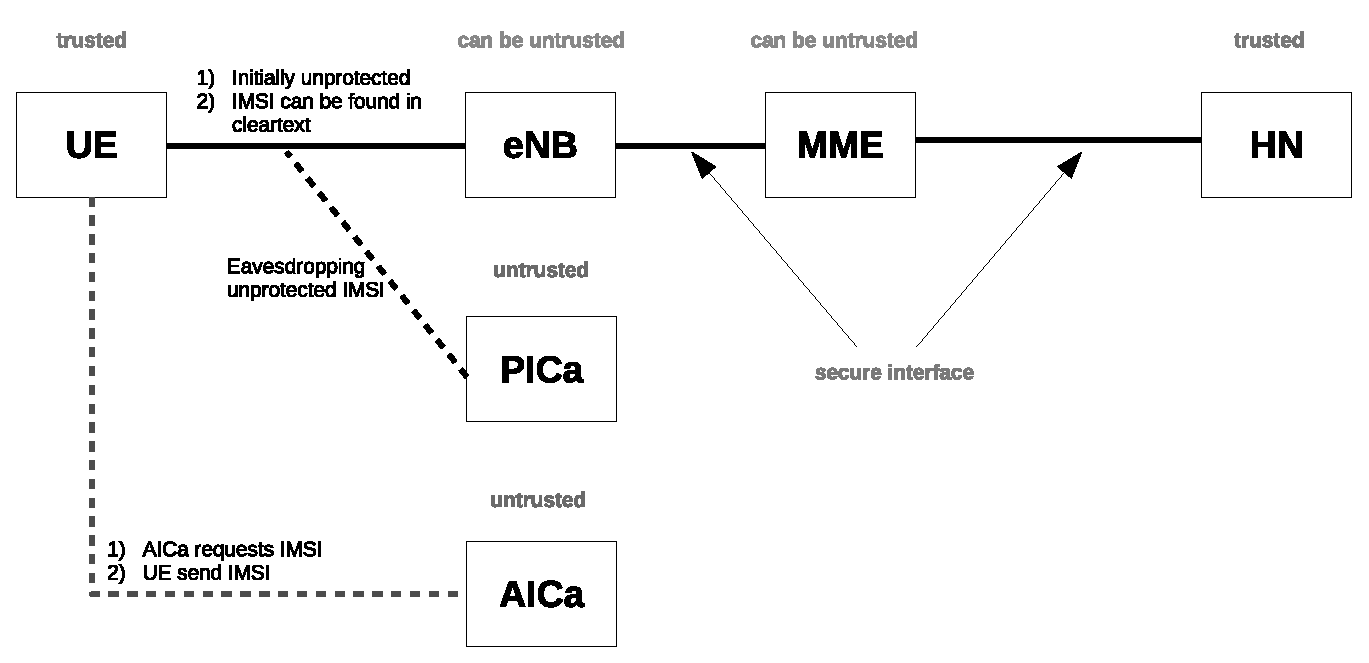
\includegraphics[width=.98\textwidth]{security_architecture_abstraction.eps}
% figure caption is below the figure
\caption{High-level security architecture}
\label{fig:security_architecture_abstraction}       % Give a unique label
\end{center}
\end{figure}

\paragraph{}
One approach of protecting IMSI privacy is to use a temporary identifier instead of the actual IMSI and keep changing the temporary identifier at a feasible frequency. Note that the temporary identifier has to be assigned over a confidentiality protected channel and different entities of the network may assign different temporary identifiers to the user equipment (UE). In the LTE network, the temporary identifier assigned by serving network (SN) is called globally unique temporary identity (GUTI) and the home network (HN) does not assign any temporary identifier to the UE. However, during the initial attachment of a UE to the SN, the UE has neither a GUTI nor a security context with the SN that can assign it with a GUTI. Besides, GUTI can be lost by either one or both of the UE and the SN. This would force the UE to reveal its IMSI to the SN to keep itself from permanently locked out of the network. This problem gives an opportunity to an active IMSI catcher (AIC) who impersonates a legitimate SN and forces the UE to run the initial attachment protocol. This also gives an opportunity to a passive IMSI catcher (PIC) to eavesdrop the IMSI sent in clear text. Solutions \cite{pseudonym_valtteri_philip, pseudonym_ericsson} have been proposed by using temporary IMSI known as pseudonym assigned by the HN. While these solutions solve the cases of lost and unsynchronised GUTI, they still have the problem of lost or unsynchronised pseudonyms and also initial attachment.
\paragraph{}
In this report we present how a security context can be set up in between the network (either SN or HN) and the UE even before the identification of the UE so that the UE can use the security context to send its IMSI with confidentiality protection. Such a security context will mitigate the attack mounted by a PIC. In addition to this, we show that an AIC would not be able to agree on a legitimate security context with the UE and consequently will not be able to find out the IMSI.
\paragraph{}
We propose different solutions based on public-key encryption that make the UE-SN interface protected even during the initial attachment in order to fight against the PIC. Our solutions also stop the AIC from running a legitimate protocol successfully that could force the UE to reveal the IMSI. However, there are other 5G requirements which our solutions should also meet. Reduced signalling overhead, improved control plane latency are two such requirements. Concealing all the parts of IMSI, namely, MCC, MNC and MSIN has been identified as another requirement. Also, in the case of public-key, the complexity involved in setting a PKI and revocation of a public-key need to be considered with high importance. In some cases the public key of an entity is pre-provisioned to all the potential senders in the system. If this public key is revoked and a new public-private key pair is generated by the entity from which the public key was revoked, then the new public key needs to be re-provisioned to all those entities that were pre-provisioned with the old public key. Considering all these requirements, we evaluate our solutions based on the following criteria:
\begin{enumerate}
\item Concealed from PIC, AIC, SN
\item Parts of the IMSI concealed
\item Signalling overhead
\item Latency
\item PKI complexity
\item Public-key revocation and re-provisioning 
\end{enumerate}
\paragraph{}
We also want to see if any of these solutions would work in a heterogeneous situation where one or more of the entities involved would come from the legacy networks. Apparently, none of the legacy networks use public-key encryption. On the other hand, all of the solutions presented in this report use public-key encryption. Therefore, it can be said that none of the solutions presented in this report will work in such a heterogeneous situation. While the choice of the solution is dependent on how much we want to achieve, hybrid solution using identity based public-key encryption and pseudonyms appear to be a promising approach.
\paragraph{}
In Section \ref{sec:id_based_crypto} we present a quick introduction to the different kinds of public-key encryption we have used in this report. In Section \ref{sec:solutions} we present the solutions based on different kinds of public-key encryption. In Section \ref{sec:evaluation}, we present an evaluation of the presented solutions based on the aforementioned evaluation criteria. Finally we conclude the paper in Section \ref{sec:conclusion}.

\section{Identity Based Encryption (IBE) in the Jargon of Encryption} \label{sec:id_based_crypto}
Modern-day encryption can be broadly categorized into two categories depending on how the keys are used to encrypt and decrypt the message. In symmetric-key encryption the sender and receiver share a secret key which is used for both encryption and decryption. In public-key encryption the receiver has a pair of keys. One of the keys is public and the other is private. The public key is used by the sender to encrypt the message and the private key is used by the receiver to decrypt the message. While the challenge in symmetric key encryption is to create a key known only by the sender and receiver but no one else, one major challenge in public-key encryption is to authenticate the public key.
\begin{figure}
\begin{center}
% Use the relevant command to insert your figure file.
% For example, with the graphicx package use
  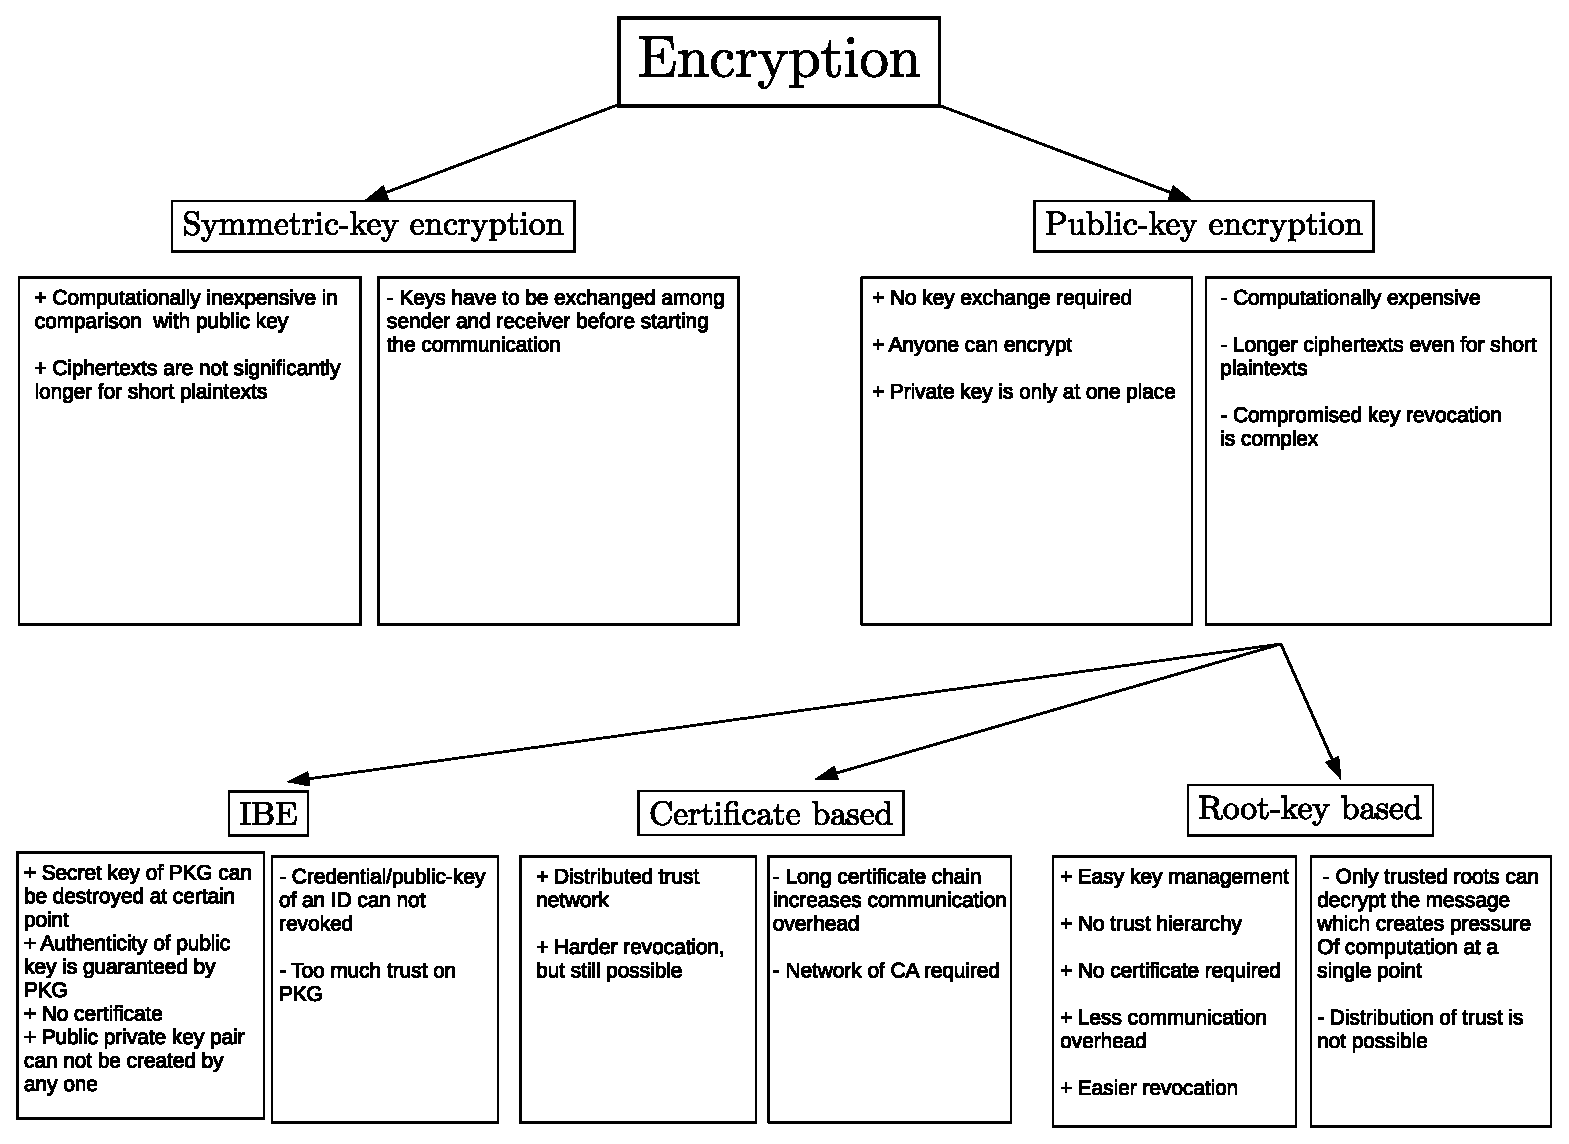
\includegraphics[width=.98\textwidth]{ibc_in_jargon_of_crypto.eps}
% figure caption is below the figure
\caption{IBE in the Jargon of Encryption}
\label{fig:ibe_in_the_jargon_of_cryptography}       % Give a unique label
\end{center}
\end{figure}
\paragraph{}
Public-key encryption can be further categorized into three more subcategories based on the authentication mechanism used to verify the public keys:
\begin{enumerate}
\item Certificate based encryption
\item Root-key based encryption
\item IBE
\end{enumerate} 
Figure \ref{fig:ibe_in_the_jargon_of_cryptography} shows this categorization with advantages and disadvantages of the respective categories. Please note that this classification is drawn considering only the encryption operation. Different classifications could be drawn based on other cryptographic operations for example digital signature, hashing or MAC. Nonetheless, we use this classification, because encryption is the most relevant cryptographic operation for identity confidentiality. We want to come up with at least one solution using each of the possible subcategories of public-key encryption. We believe all public-key encryption based solution fall into one of these three subcategories with high probability. It makes sense to first compare categories and only in the second phase, compare individual solutions inside each category. We also believe, this is a systematic approach which makes the comparative evaluation easier and meaningful.
However, we do not dig deep into within-category comparison in this report.
\paragraph{}
In the certificate based encryption, the public key is signed by a trusted third party. The sender of the message has to be pre-provisioned with the root certificate so that the sender can authenticate the public key of the receiver. In the root-key based encryption, no runtime authentication of the public key is required, because a very limited number of public keys are used in the system and all the senders are pre-provisioned with all the existing public keys. In IBE, the public key of a receiver is computed from the identity of the receiver and the public key of a trusted third party. The public key of the trusted third party has to be provisioned to sender. The private key of the receiver is computed from the identity of the receiver and the private key of the trusted third party. The private key of the receiver has to be provisioned to the receiver by the trusted third party.
\paragraph{}
In the next section we present solutions based on different public-key encryption schemes. While presenting the solutions we will discuss more about how these different kind of public-key encryption works.

\section{Solutions}\label{sec:solutions} 
\label{sec:solutions}
It is beneficial to introduce some notation here before delving into the solutions. 
\begin{enumerate}
\item $hnid=MCC||MNC$ identifies the HN
\item $snid=MCC||MNC$ identifies the SN
\item $e_A$ is the public key of entity $A$
\item $d_A$ is the private key of entity $A$ 
\item $\mathcal{X}_{A,B}(e_A,e_B)$ is the certificate of the public key $e_A$ of $A$. The certificate can be verified by anyone who considers $B$ as a root CA using the public key $e_B$. The certificate is a guarantee from B that the public key $e_A$ is owned by $A$ .
\item $E,D$ are the encryption and decryption functions, respectively.
\end{enumerate}


\subsection{Solution Based on Certificate Based Public-key Encryption} 
\label{sub_sec:solution_certificate}
In certificate based public-key cryptography, certificates digitally signed by trusted third parties are used to authenticate the ownership of a public key. A trusted third party who can sign a certificate is called a certificate authority (CA). It is possible to build a chain of trust in certificate based public-key cryptography by allowing an entity to become a CA who is certified by another CA. A certificate contains a digital signature which allows anyone to verify the validity of the certificate by verifying the digital signature using the public key of the CA who issued the certificate. There has to exist at least one CA in a chain of trust whom the verifier already trusts. There might exist entities who certify themselves and some verifiers trust these entities. The entities having self signed certificates who are trusted by verifiers are considered as the root CAs for those verifiers and the corresponding certificates are called root certificates. 
\subsubsection{Description}
To use certificate based public-key cryptography to secure IMSI privacy, we need to figure out a few things first: who are the root CAs and who else can be a CA, who are the entities that own a public key, how a certificate can be revoked, and how the UE can be re-provisioned with a new root certificate if required.
\paragraph{}
We choose the HN of a subscriber as the root CA for the subscriber. This is a reasonable choice, because in any case the HN knows the IMSI of a subscriber. This is because it is the HN which has chosen the IMSI in the first place. So, the HN is entrusted with the IMSI itself. As a result the choice of entrusting the HN with the key which protects the IMSI is reasonable. HN owns a self signed certificate which is the root certificate. Every UE having a subscription of the HN is provisioned with the root certificate. An SN owns a public key certified by HNs. 
\paragraph{}
The solution has three different phases as presented in Figure \ref{fig:solution_certificate}. In the provisioning phase the network generates public-private key pair and provisions the public key to all its subscribers. As shown in step $1$ of this phase, the HN generates a public-private key pair and generates a certificate of the public key signed by the HN itself.  In step $2$, a UE is provisioned with the self signed certificate which was generated in step $1$. Please note that step $1$ is performed when HN is installed. Step $2$ is performed when a UE is provisioned with the subscription of the HN. However, in case of compromised private key of HN, the provisioning phase (both step $1$ and $2$) is required to be performed again. We will discuss this issue later in this subsection. 
\paragraph{}
During the roaming agreement in between two networks, the SN obtains a certificate from the HN. In step $1$ of this phase, the SN sends its public key $e_{snid}$ and $snid$ to the HN. The HN generates a certificate $\mathcal{X}_{snid,hnid} (e_{snid},e_{hnid})$. This certificate is a guarantee from the HN that the public key $e_{snid}$ is owned by the network identified by $snid$ and is verifiable by the public key $e_{hnid}$.
\paragraph{}
In the identification phase, the SN broadcasts its identity in step $1$. The UE sends $hnid,e_{hnid}$ to the SN in step $2$. In step $3$, the SN looks up for the certificate $\mathcal{X}_{snid,hnid} (e_{snid},e_{hnid})$. In case it exists at the disposal of the SN, the SN sends $\mathcal{X}_{snid,hnid} (e_{snid},e_{hnid})$ to the UE in step $4$. The UE verifies the certificate in step $5$ and extracts the public key $e_{snid}$ from the certificate. If the certificate is verified as valid, then the UE sends the IMSI to the SN encrypted by the public key of the SN in step $6$. To avoid the ciphertext to be the same every time, the UE concatenates a $salt$ at the end of the IMSI of agreed length before encrypting. SN decrypts the ciphertext, discards the salt from the tail and extracts the IMSI. This completes the identification of a UE to the SN. Figure \ref{fig:solution_certificate} shows the protocol in detail. Note that in the roaming agreement phase the SN does not need to get the certificate from the HN, but the SN can get it from any CA who is trusted in by the HN in the chain of trust.
\begin{figure}
\begin{center}
% Use the relevant command to insert your figure file.
% For example, with the graphicx package use
  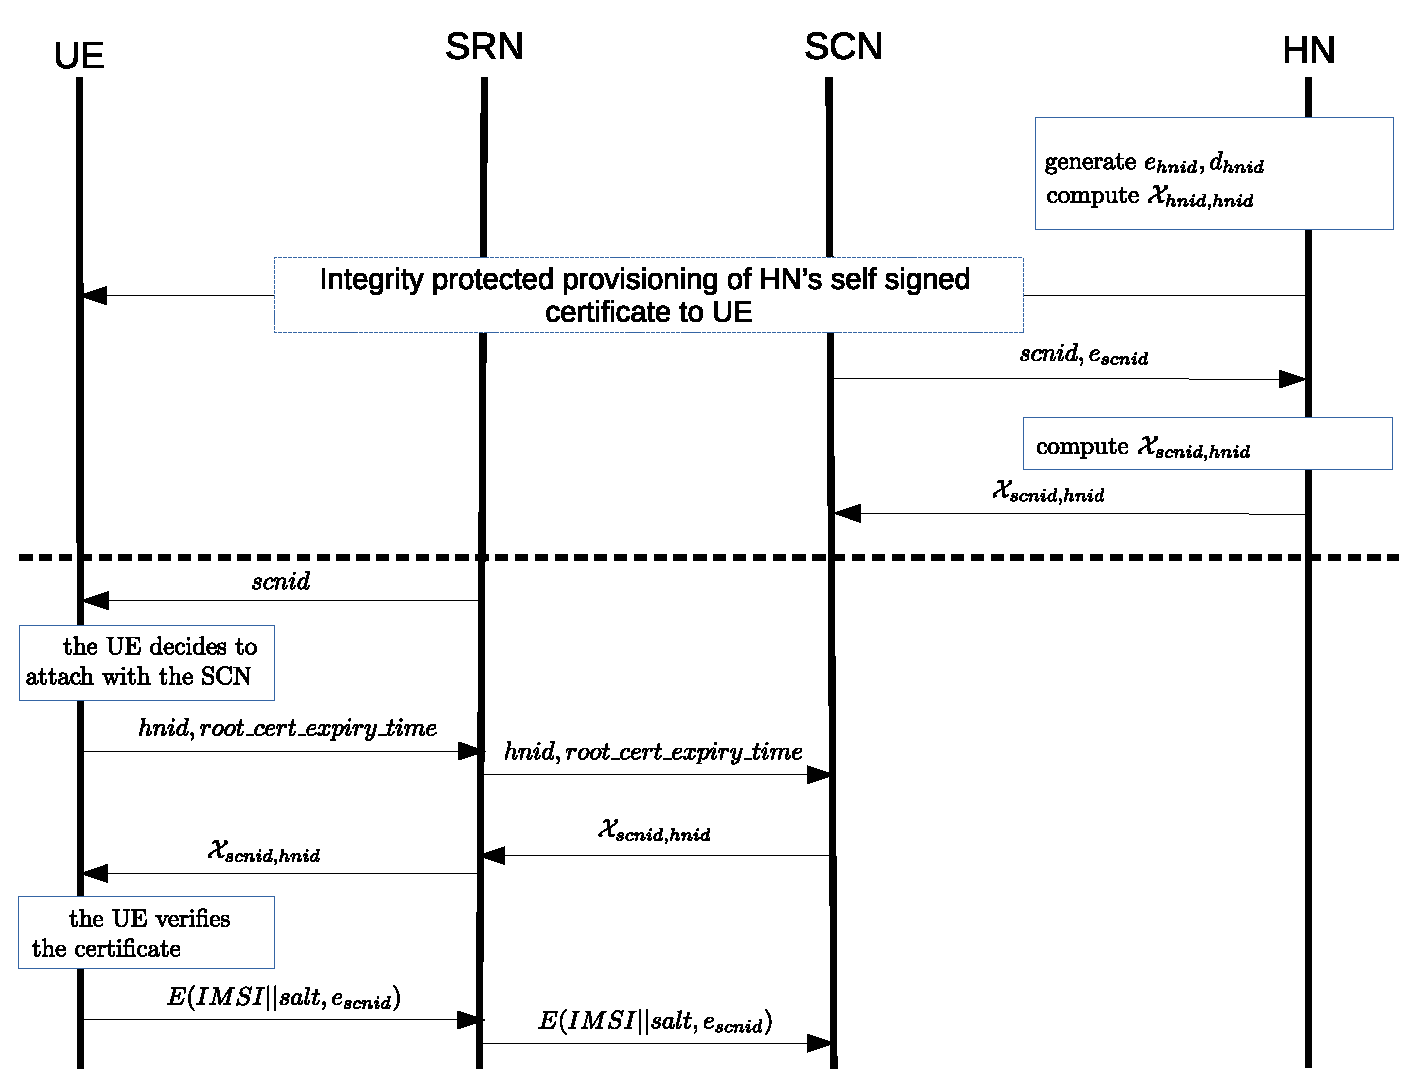
\includegraphics[width=.98\textwidth]{public_key_variation1.eps}
% figure caption is below the figure
\caption{Privacy protected UE identification using certificate based public-key encryption}
\label{fig:solution_certificate}       % Give a unique label
\end{center}
\end{figure}
\subsubsection{Revocation of the Public Keys of SNs}
Every CA in the system maintains a list of revoked public keys which were certified (at the first place) by it or by any other CA trusted by it. If there is a revocation, the CA who provided the certificate at the first place updates its revoked list and the CA updates its CA with the information. The UE periodically runs a protocol with the HN to download the latest revoked public keys. If a dishonest SN presents a UE with the certificate which is already revoked but the UE has not yet been able to download it, then the MSIN will be revealed to the dishonest SN. However, such a dishonest SN will fail to run a successful authentication protocol. As soon as the UE comes in touch with a legitimate SN, it identifies itself successfully, runs a successful authentication protocol, and downloads the latest revocation list from the HN. Thereafter the dishonest SN will not be able to reveal the MSIN any more. This implies that an AIC can mount an attack if it was once trusted by the HN as a legitimate SN but is no more trusted by the HN and the UE is not yet updated with the withdrawal of the trust. The existence of such an AIC is apparently extremely rare. The time window this attack allows to track a subscriber is also very small. Altogether this makes the attack expensive. However, if the private key of an SN is stolen, both PIC and AIC can mount attacks until the public key is revoked. 
\subsubsection{Revocation of the Public Key of the HN}
Consider the situation when the private key of the HN is compromised but the subscription details of the subscribers' are still secure for some reason. Such a partial security breach of the HN is possible if e.g. the private key is kept in a different server than the one where the subscription details are stored. The entity which has an access to the compromised private key can mount an attack as an AIC. The HN can recover from this situation by updating itself with a new public-private key pair and generating a new root certificate. Every UE that has a subscription with the HN needs to be re-provisioned with the new root certificate. Whenever the public-private key pair of a CA (HN is a CA) is revoked by a new pair, all the certificate chains becomes invalid in which there is a certificate signed by the revoked key of the CA. In this case all those entities to which the invalid certificate chain was issued has to get a new valid certificate chain. 
\paragraph{}
However, there is a synchronization issue which needs to be considered in this regard. The synchronisation can happen in three different ways: 
\begin{enumerate}
\item None of UE and SN are updated with the change in HN
\item SN is updated with new valid certificate chain but UE is not provisioned with the new root certificate
\item UE is provisioned with new root certificate but SN is not updated with a new valid certificate chain
\end{enumerate} 
\paragraph{}
In the first case the entity who has access to the HN's compromised private key can attack as both PIC and AIC. These attacks can be successful until the UE and SN are updated with the required changes because of the new public key of HN. In the second case, if an SN is updated with a valid certificate chain and the UE does not have the new root certificate, then the UE will never be able to verify the certificate presented by a legitimate SN. To circumvent this problem the SN stores certificates chained with all the root certificates used by an HN. The SN first checks the $e_{hnid}$ sent by the UE. The SN then finds the certificate chain provided by the HN in which the root certificate is of $e_{hnid}$ and sends this particular certificate to the UE. Once the UE is attached to a legitimate SN, the HN can send the new root certificate to the UE with authenticity and integrity protection. Another way is to publish the new root certificate in the public media with integrity protection so that anyone can download the root certificate using some other internet connection. In the third case, if the UE is updated with the latest public key of the HN but the SN is not, then the SN will not be able to provide a valid certificate to the UE. In such a case, the SN has to ask the HN to issue a certificate to SN's public key which would be verifiable by the new public key of HN. We have not presented the solution of the third case in the figure.
\paragraph{}
The need for re-provisioning the UE with a new root certificate might be an extremely rare event. Besides, once the need for existing root certificate revocation and provisioning of a new one is identified, it does not allow the attacker a long time window to track the UEs. However, protecting the confidentiality of a private key and detecting the compromise of a private key is a whole different security question and we do not delve into that in this report.
\subsubsection{Pros and Cons}
This approach can not conceal $hnid$. It conceals MSIN from AIC, PIC. The IMSI is revealed entirely at SN. It requires a full round trip signalling in between UE and SN before sending the encrypted MSIN. It carries $hnid$ from UE to SN and in return carries the public-key certificate back from SN to UE. Public keys are quite large, length of a minimum ciphertext is also very long comparatively, and the certificate chain can be quite long. Consequently it adds significant signalling overhead. Also, public-key cryptography is computationally heavier than that of symmetric-key cryptography. As a result, latency will increase significantly to verify the certificate and encrypt the IMSI. Nevertheless, once a UE is identified by the network, the network assigns a GUTI to the UE. It is a question for further research to evaluate the effect of this extra signalling overhead and increased latency. This solution does not work in a heterogeneous situation when any of the involved entities come from legacy networks. On the other hand, it does not require to establish any new trusted authorities. Hence, PKI complexity is very little. Revocation of the public-key of an SN and an HN is possible and complex.


\subsection{Solution Based on Certificate Based Public-key Encryption with a Very Short Trust Chain} 
\label{sub_sec:solution_certificate_short_chain}
\subsubsection{Description}
The use of a very short trust chain is exactly the same mechanism as described in section \ref{sub_sec:solution_certificate} except that only a HN can be a CA. As a result the chain of trust is very short and consequently the certificate chains are also very short.  Figure \ref{fig:solution_certificate_short_chain} shows the protocol in detail. 

\subsubsection{Revocation of the Public keys of SNs and the HN}
As only an HN is a CA, the complete revocation list of public keys is found in HN at any point of time. Whenever the UE is attached to a legitimate network, it can download the revocation list from the HN. If the HN's public key need to be changed and provisioned again to the UE, it can be done in the same way as discussed in \ref{sub_sec:solution_certificate}.

\begin{figure}
\begin{center}
% Use the relevant command to insert your figure file.
% For example, with the graphicx package use
  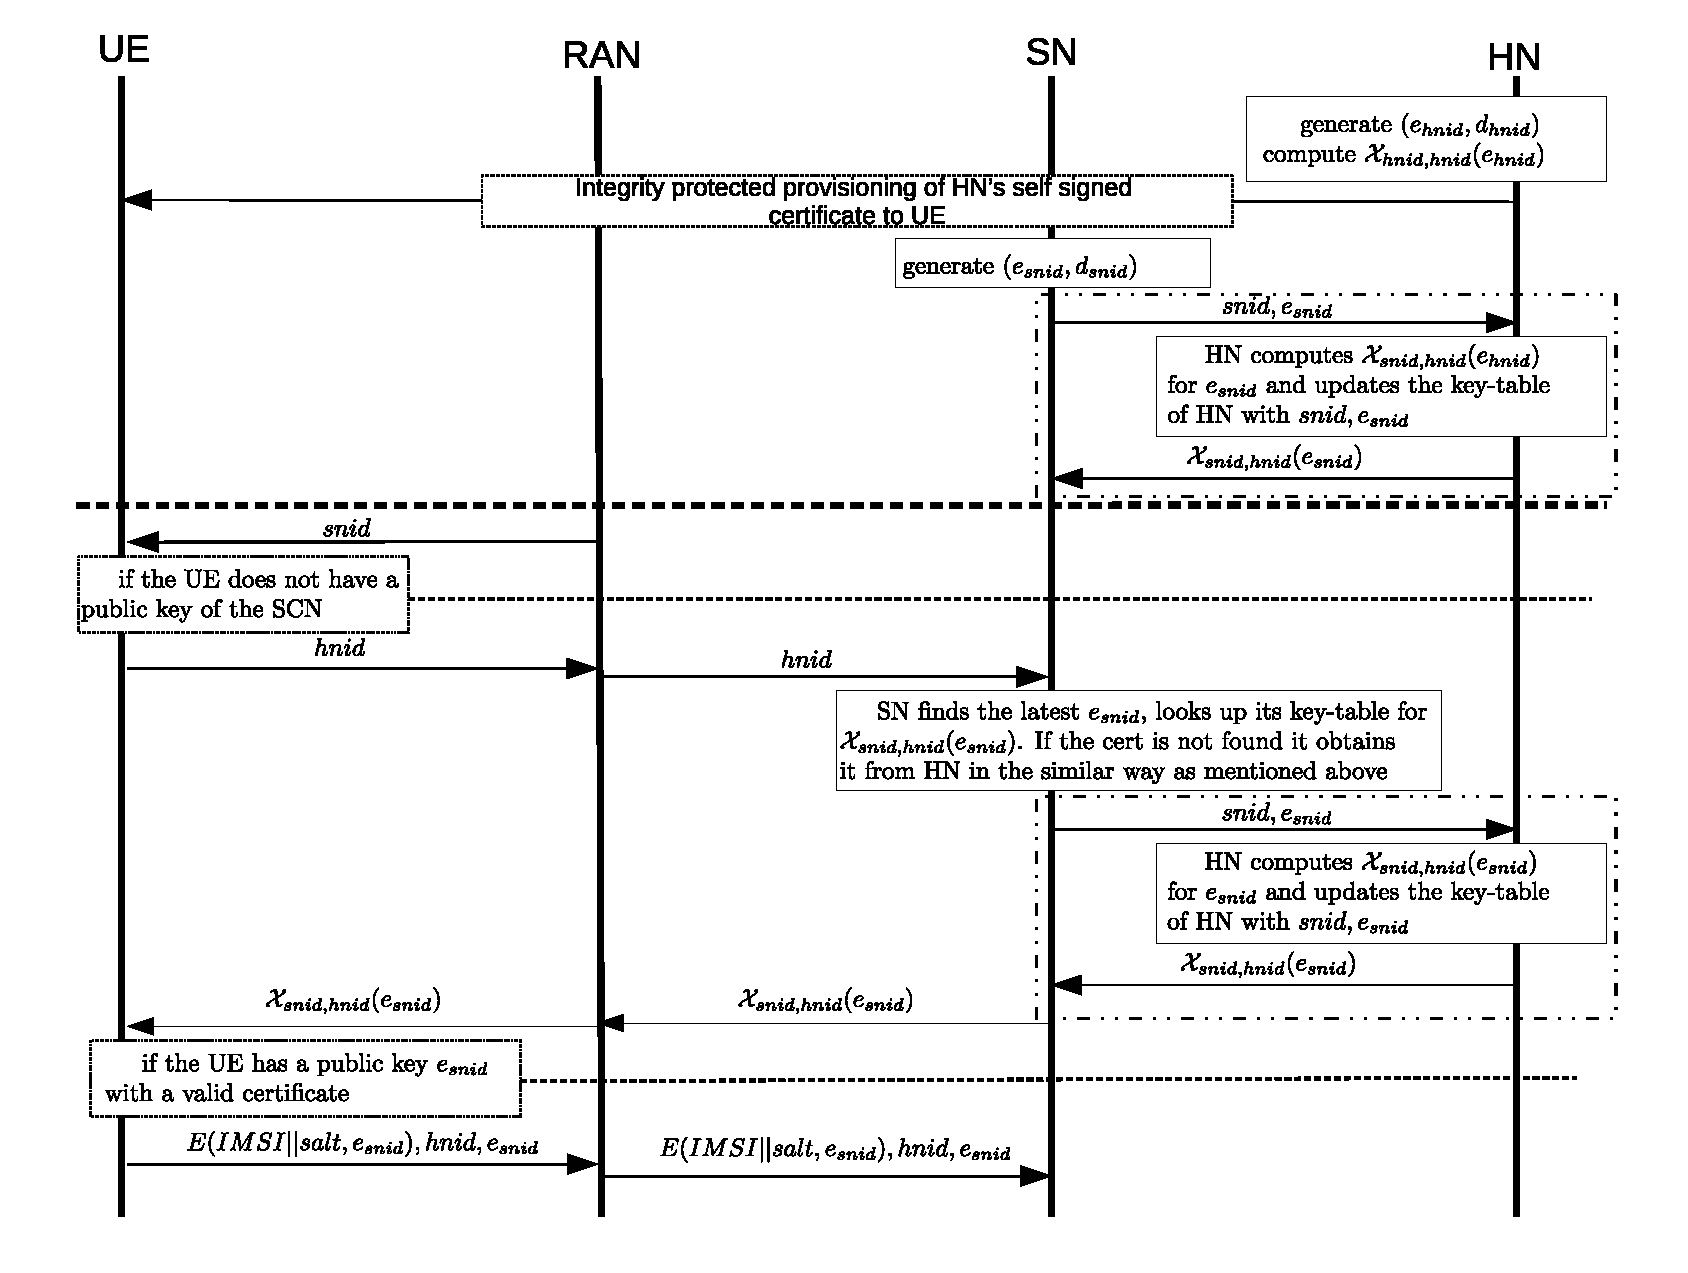
\includegraphics[width=.98\textwidth]{root-key2.eps}
% figure caption is below the figure
\caption{Privacy protected UE identification using certificate based public-key cryptography with a short trust chain}
\label{fig:solution_certificate_short_chain}       % Give a unique label
\end{center}
\end{figure}

\subsubsection{Pros and Cons}
This approach can not conceal $hnid$. It conceals MSIN from AIC, PIC. The IMSI is revealed entirely at SN. Unlike the solution in \ref{sub_sec:solution_certificate}, this approach may not require a full round trip signalling in between UE and SN before sending the encrypted MSIN. However, this protocol has the downside of heavy computational requirements and signalling overhead due to the large size of public keys and ciphertext. Due to short certificate chains, it reduces the signalling overhead and computational latency comparatively. Revocation of the public keys of SNs and the HN is possible and comparatively easier. 
\paragraph{}
The burden of exchanging the certificates and verifying them can be avoided to some extent by periodically provisioning the UE with the public key of the probable SNs the UE might visit in near future. The solution presented in Section \ref{sub_sec:solution_certificate_short_chain_pre-provisioned_keys} is motivated by this idea.

\subsection{Solution Based on Certificate Based Public-key Encryption with a Very Short Trust Chain and Pre-provisioned Public Kyes of SNs} 
\label{sub_sec:solution_certificate_short_chain_pre-provisioned_keys}
\subsubsection{Description}
The UE is periodically provisioned by the HN with the public key of the probable SNs the UE might visit in near future. If the SN asks for the IMSI from the UE, the UE looks for a public key of the SN in the key-table of the UE provisioned by HN. If it finds a public key $e_{snid}$, it encrypts the IMSI with the public key and sends the ciphertext to the SN along with $e_{snid}$ without asking a certificate for the public key from the SN. With these modifications the protocol evolves to the one presented in Figure \ref{fig:solution_certificate_root_key_hybrid}.
\begin{figure}
\begin{center}
% Use the relevant command to insert your figure file.
% For example, with the graphicx package use
  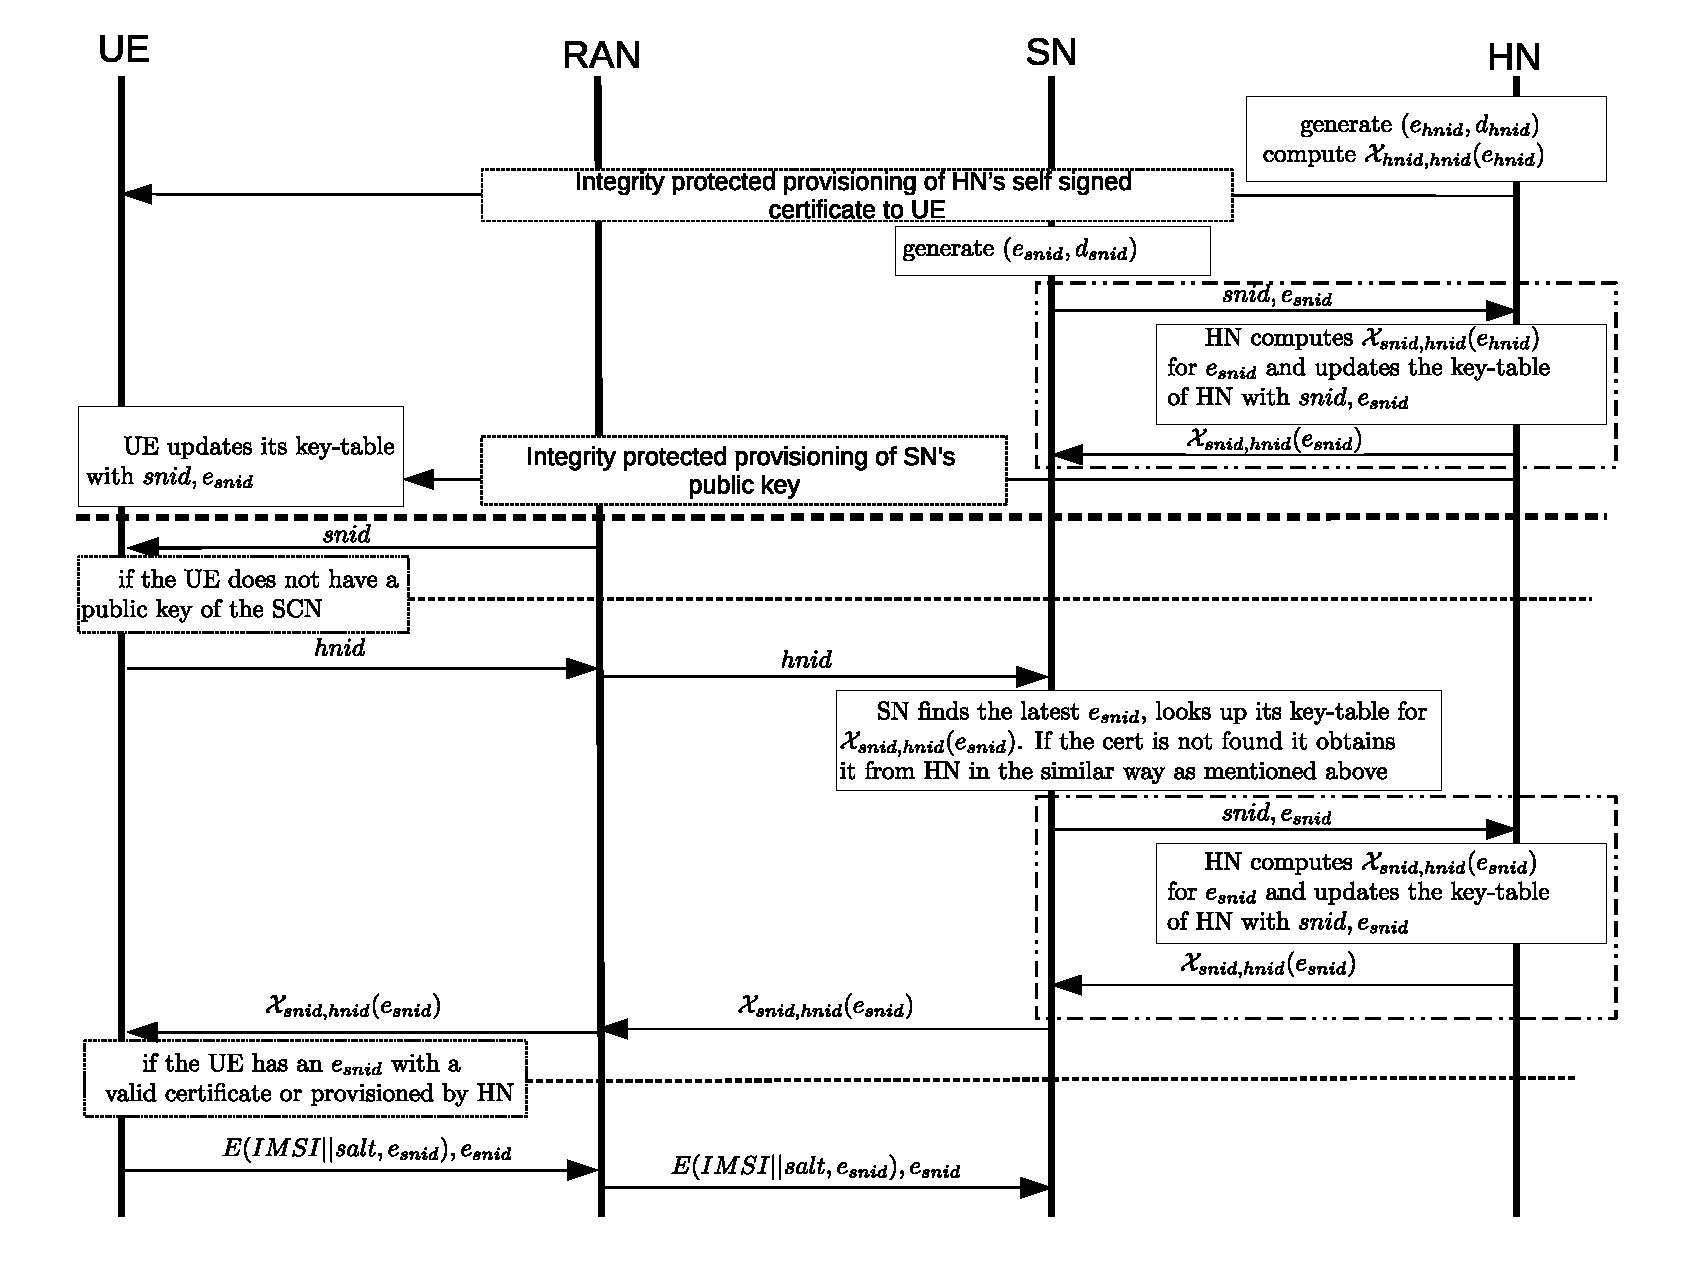
\includegraphics[width=.98\textwidth]{root-key3.eps}
% figure caption is below the figure
\caption{Privacy protected UE identification using certificate based public-key cryptography with a short trust chain and pre-provisioned public keys of the SNs}
\label{fig:solution_certificate_root_key_hybrid}       % Give a unique label
\end{center}
\end{figure}


\subsubsection{Revocation of Public Keys of SNs and the HN}
As only an HN is a CA, the complete revocation list of public keys is found in HN at any point of time. Whenever the UE is attached to a legitimate network, it can download the revocation list from the HN. If the HN's public key need to be changed and provisioned again to the UE, it can be done in the same way as discussed in \ref{sub_sec:solution_certificate}.

\subsubsection{Pros and Cons}
This approach can not conceal $hnid$. It conceals MSIN from AIC, PIC. The IMSI is revealed entirely at SN. Unlike the solution in \ref{sub_sec:solution_certificate}, this approach might not require a full round trip signalling in between UE and SN before sending the encrypted MSIN. If an SN is likely to be visited by a UE, the HN will most likely provision the UE with the public key of the SN. Hence, the exchanges of certificates are most likely the cases when AICs are asking for the IMSI. In such a case, the cost of heavy computation and signalling overhead can be considered as the price of detecting AICs. 
However, this protocol still has the downside of heavy computational requirements and signalling overhead due to the large size of public keys and ciphertext. Revocation of the public keys of SNs and the HN is possible and comparatively easier. 




\subsection{Solution based on Root-key based Encryption} 
\label{sub_sec:solution_root-key}
\subsubsection{Description}
In root-key based public-key encryption, there is only a very limited number of public-private key pairs in the network. All the senders in the network are pre-provisioned with the public key of the receivers. We use only one pair of public-private key pair in the approach. This key pair is owned by the HN and we call it to be the root-key. The public key is provisioned to all the UE by the HN which have subscriptions with the HN. Whenever a UE is in need of identifying itself to a SN with the IMSI, the UE encrypts the IMSI with the public root key and sends the result to the SN along with the $hnid$. Note that the UE concatenates a random $salt$ of agreed length at the end of the IMSI before encryption to avoid having the same encrypted IMSI every time. The SN sends the encrypted IMSI to the appropriate HN. The HN decrypts and extracts the IMSI. To facilitate LI, the HN sends back IMSI to SN. Figure \ref{fig:solution_root-key1} shows the protocol in detail.

\begin{figure}
\begin{center}
% Use the relevant command to insert your figure file.
% For example, with the graphicx package use
  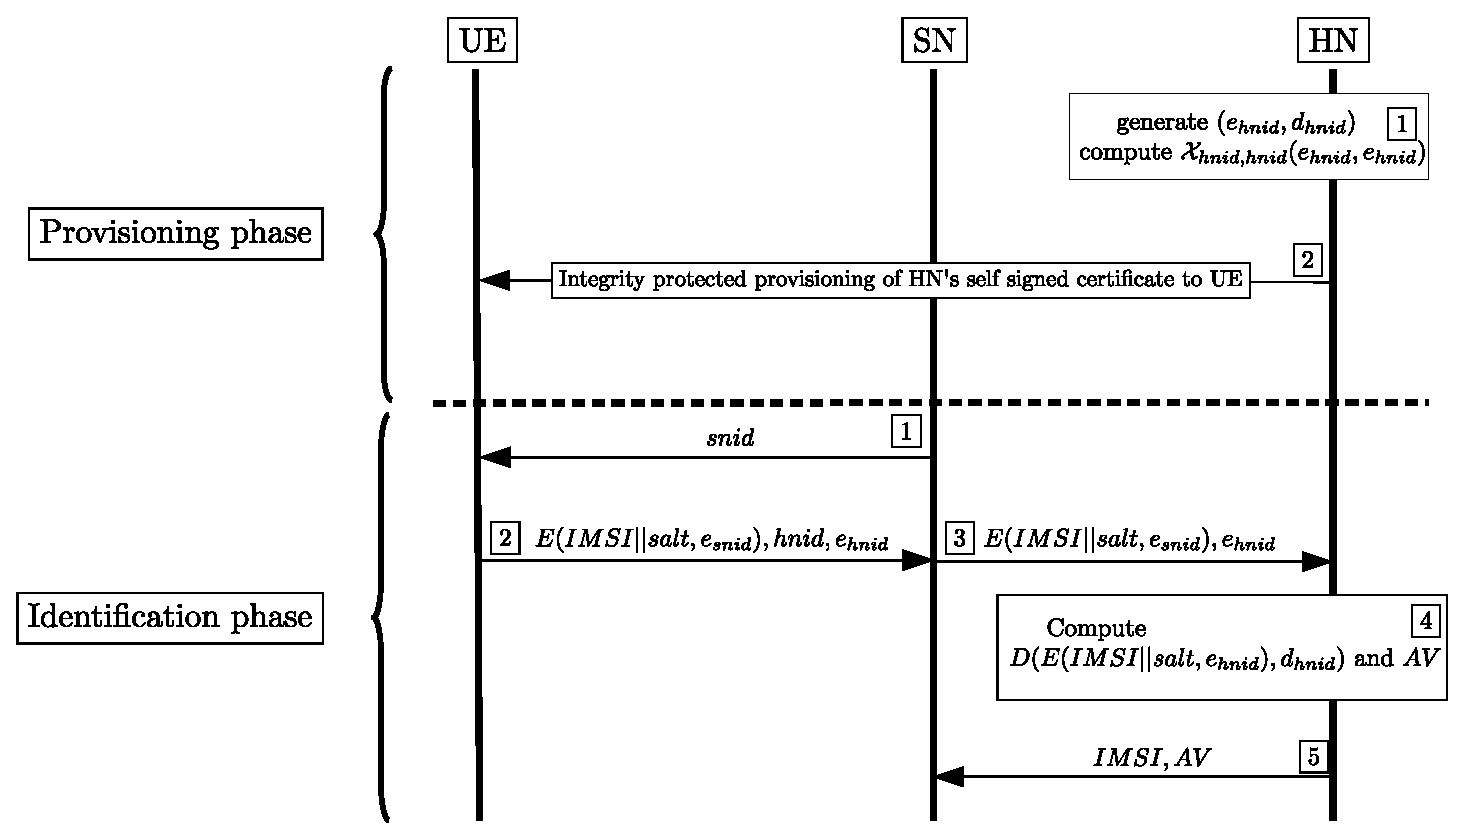
\includegraphics[width=.98\textwidth]{root-key1.eps}
% figure caption is below the figure
\caption{Privacy protected UE identification using a single root-key}
\label{fig:solution_root-key1}       % Give a unique label
\end{center}
\end{figure}

\subsubsection{Revocation of the Root-Key}
Consider the situation when the root-key in HN is compromised but the subscription details of the subscribers' are still secure for some reason. Such a partial security breach of the HN is possible if e.g. the root-key is kept in a different server than the one where the subscription details are stored. To recover from this situation, the HN generates a new pair of keys. All the UEs of the HN has to be re-provisioned with the new public key. If not, then someone who has access to the compromised private key will be able to eavesdrop the encrypted IMSI and decrypt it. Also someone who gets access to the compromised private key will be able to mount an attack as an AIC. However, if the public key in the HN is changed and a UE not provisioned with the new public key sends the encrypted IMSI to the HN via a legitimate SN, the HN will not be able to decrypt it with the new private key. To circumvent this problem, the HN stores all the public-private key pair it has ever used. When UE sends the encrypted IMSI, it also sends the public key that was used for the encryption. In this way, the HN knows which private key should be used decrypt the IMSI. 

\subsubsection{Pros and Cons}
This approach can not conceal $hnid$. It conceals MSIN from AIC, PIC. The IMSI is revealed entirely at SN. However, it is in principle possible that the HN would provide a fake IMSI of the subscriber to the SN. In that case the requirement of LI would not be fulfilled. Nevertheless, even if the HN provided the genuine IMSI of the subscriber, the LI authority would need the HN to cooperate by revealing the identity of the subscriber. So, hence we trust that the HN would cooperate with LI, it is reasonable to trust that the HN would not provide a fake IMSI to the SN. This solution does not need to transfer and verify the certificate each time the protocol is run. This approach reduces the signalling and computational overhead compared to the certificate-based approach. However, the problems of heavier computation for public-key encryption and large ciphertext expansion remain as downsides of this solution.  Nevertheless, once a UE is identified by the network, the network assigns a GUTI to the UE. It is a question for further research to evaluate the effect of these downsides in signalling overhead and increased latency. This solution does not require to establish any new trusted authorities, so there is no PKI complexity involved. Public key revocation is possible and easy.


\subsection{Solution based on IBE} 
\label{sub_sec:solution_ibc}
As already mentioned in Section \ref{sec:id_based_crypto}, in IBE the public and private key of a receiver is computed from the identity of the receiver in conjunction with the public and private key of a trusted third party respectively. As the private key of the trusted third party is required to compute the private key of the receiver, the private key of the receiver has to be provisioned to the receiver by the trusted third party. Even though an extra one-time burden of private key provisioning is required, a sender does not need to authenticate the public key of a receiver each time the sender and the receiver agree on a security context. The sender does not need to authenticate the public-key, because if the public key is not authentic, the receiver will not have the private key. If the receiver does not have the private key, any message encrypted by the public key will never be decrypted by the receiver. On the other hand the private key of the receiver would be provisioned to the receiver only if the receiver can authenticate itself to the trusted third party. In other words, the authenticity of the public key in IBE is guaranteed by the trusted third party. Usually in IBE, the trusted third party is known as the private key generator (PKG). While in the certificate based and root-key based cases it is possible to revoke the public key of a receiver, it is impossible to revoke the public key in IBE unless the identity itself is revoked. Please note that, a PKG knows the private keys of all the receivers whose public keys were generated using the PKG's public key. As a result a PKG can decrypt any message sent by any sender to any receiver. This assumes a very high level of trust in the PKG.  In Figure \ref{fig:how_ibc_works}, we show how IBE works pictorially.


\begin{figure}
\begin{center}
% Use the relevant command to insert your figure file.
% For example, with the graphicx package use
  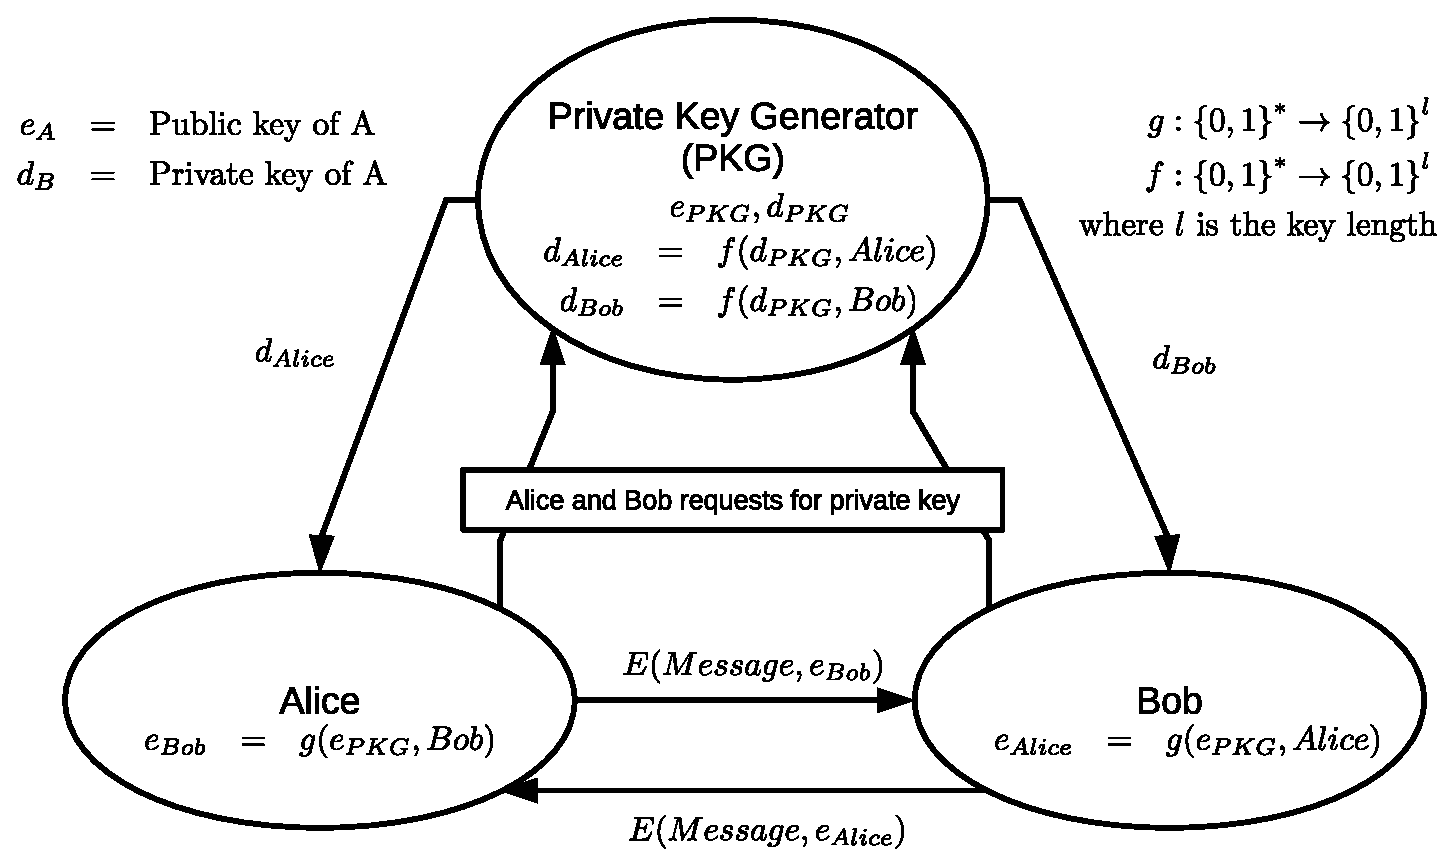
\includegraphics[width=.98\textwidth]{how_ibc_works.eps}
% figure caption is below the figure
\caption{IBC mechanism}
\label{fig:how_ibc_works}       % Give a unique label
\end{center}
\end{figure}

\begin{figure}
\begin{center}
% Use the relevant command to insert your figure file.
% For example, with the graphicx package use
  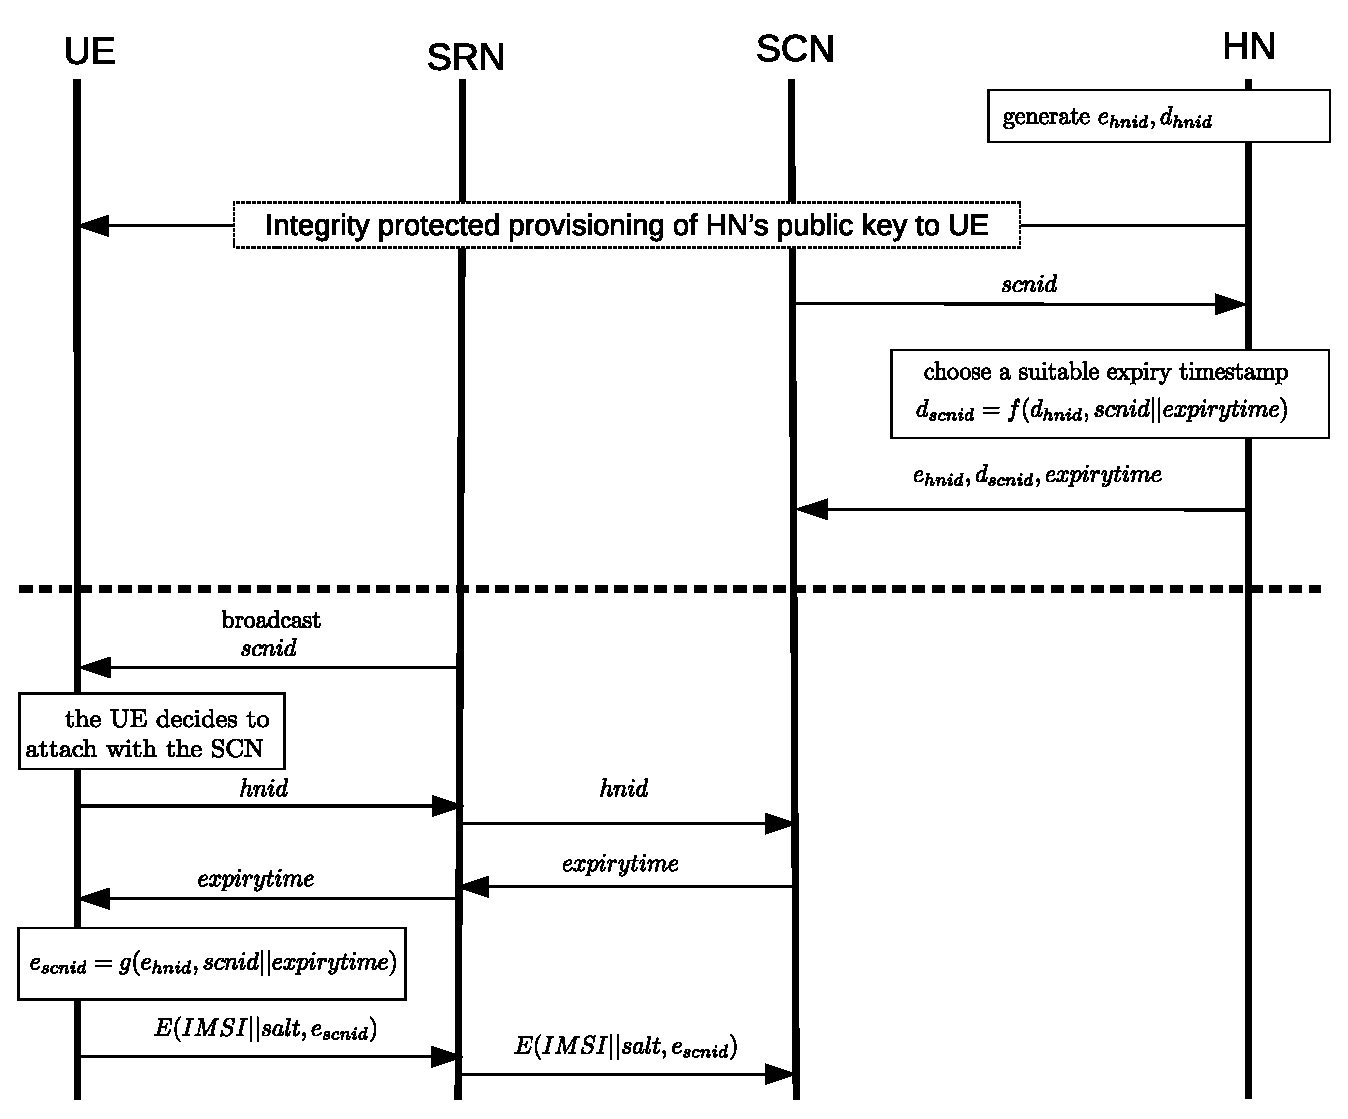
\includegraphics[width=.98\textwidth]{solution_based_on_ibc.eps}
% figure caption is below the figure
\caption{Privacy protected UE identification using IBE}
\label{fig:solution_ibc}       % Give a unique label
\end{center}
\end{figure}

\subsubsection{Description}
In this approach, a UE is considered as the sender. The SN a UE is trying to connect with, is considered as the receiver. The UE's HN acts as the PKG. The HN is trusted as the PKG because the UE is a subscriber of the HN and the UE trusts the HN with the IMSI in all the legacy networks. In all the legacy networks, the HN can technically mount both of the PIC and AIC attacks against its subscribers. Still it is trusted that the HN would not mount an IMSI catcher attack. On the other hand, choosing the HN as PKG gives the HN the ability to decrypt any encrypted IMSI sent by a UE to an SN. As a result an HN gets the ability to become a PIC or an AIC. Consequently, choosing the HN as PKG does not increase level of trust required in an HN comparing with the approaches used in all the legacy networks. Please note that an SN may serve many UEs coming from different HNs. Hence, an SN can have different public-private key pairs associated with different HNs. 
\paragraph{}
The solution is pictorially presented in Figure \ref{fig:solution_ibc}. It has three different phases. In provisioning phase, the HN generates a public-private key pair $e_{hnid},d_{hnid}$ in step $1$. In step $2$ of this phase, the HN provisions the UE with the public key $e_{hnid}$. During roaming agreement phase, the SN sends the $snid$ in step $1$. In step $2$ the HN chooses a suitable expiry time $expirytime$ for the private key of the SN. The expiry time is appended with $snid$ and the private key $d_{snid}$ is computed considering $snid||expirytime$ as the identity of the SN. The reason for using a expiry time as part of the identity of the SN will be discussed later when we discuss the revocation of the public key of an SN. In step $3$, the HN sends $d_{snid}$ to the SN along with $expirytime$ and $e_{hnid}$. In step $4$, the SN stores these information in its key-table. In the identification phase, in step $1$, the SN broadcasts the $snid$. In step $2$, the UE sends back the $hnid$ to the SN. In step $3$ the SN extracts the $expirytime$ given by the HN from the key-table. In step $4$, SN sends $expirytime$ to the UE. In step $5$ the UE computes the public key of the SN $e_{snid}$ as mentioned in the figure. In step $6$ the UE encrypts the IMSI using $e_{snid}$ and sends the encrypted IMSI to the SN along with $e_{hnid}$. Like the other approaches, a random $salt$ of agreed length is concatenated with IMSI before the encryption to avoid having the same encrypted IMSI all the time. At this point the identification ends in a normal situation. However, the SN might need to consult further with the HN in a special case as mentioned in Figure \ref{fig:solution_ibc}. We will discuss that later in this subsection when we discuss the issue of changing the public-private key pair of the HN. 


\subsubsection{Revocation of Public Keys SNs}
As the public key in IBE can not be revoked, we use the concept of expiry time as the part of the identity of an entity. The expiry time is a time stamp in the future. Based on the level of trust the HN has in the SN, the HN chooses an expiry time for the SN before computing the private key of the SN. The same expiry time is sent to the UE by the SN. The UE checks if the expiry time is expired or not. If the expiry time is not expired, the UE uses this expiry time to compute the public key of the SN. At some suitable point of time before the expiry time, the SN asks the HN to provide with a new expiry time further in the future. If the SN is not trusted any more, the HN does not compute the private key for the SN and the old public key given to the SN expires when the expiry time comes. If the private key of the SN is compromised but the SN is still trusted by the HN, the HN computes a new private key using a new expiry time when the SN asks for a private key. Thus a compromised private key can be used by an attacker to mount an attack only until the expiry time used to compute the compromised private key. If the expiry time is chosen as a time stamp far in the future, then the revocation will take long time. If the expiry time is chosen as a time stamp quite near in the future, then the revocation will be quick. In such short expiry time, the signalling overhead in between the HN and SNs will increase. Nevertheless, this signalling overhead does not depend on the number of UEs connecting to the SN and this signalling overhead is a not in the radio network. Hence this overhead might not be very critical.  In case longer expiry time is used, a list of revoked $snid||expirytime$ can be maintained by the HN. Whenever there is a change in the list and a UE is attached to a legitimate SN, the HN can send the change to the UE with both authenticity and integrity protection. The list of revoked public key will not grow over time because after the expiry time, a public key is automatically revoked. In this way, AIC and PIC will be able to attack if the they know the private key of the SN and the breach of SN's private key is undetected by the SN. An AIC will be able to mount an attack when the AIC knows the private key of the SN and the expiry time involved in the identity of the SN is not yet expired and the UE is not yet updated with the list of the revoked public keys.
\subsubsection{Revocation of the Public Key of the HN}
Consider the situation when the private key of the HN is compromised but the subscription details of the subscribers' are still secure for some reason. Such a partial security breach of the HN is possible if e.g. the private key is kept in a different server than the one where the subscription details are stored. In such situation, the entity having access to the private key of the HN can mount attacks both as a PIC and AIC. The HN can recover from this situation by changing the public-private key pair. If the HN changes its public-private key pair, the private key of all the SNs have to be recomputed and be sent to the SNs. All the UEs have to be re-provisioned with the new public key of the HN. There are three possible cases of synchronisation.
\begin{enumerate}
\item None of UE and SN are updated with the change in HN
\item SN is updated but UE is not
\item UE is updated but SN is not
\end{enumerate} 
\paragraph{}
In the first case, the entity having access to the private key of the HN will be able to attack as AIC and PIC until the expiry time of SN comes. When the expiry time comes, the SN gets a new private key from the HN along with the new public key of the HN. This leads to the second case above. In such case the protocol continues from step $7$ of Figure \ref{fig:solution_ibc}. In step $7$, the SN finds that the UE is still using the old public key of the HN. In step $8$, the SN asks the HN to compute a private key for the SN using the old private key (the one for which the UE has the public key) of HN and the current expiry time of the SN. In step $9$, the HN checks if the public key sent by the SN is a public key used by the HN previously. If so, this indicates that there is a UE which is not yet updated with the new public key of the HN. The HN computes the private key accordingly and send it to the SN in step $10$. The SN uses this private key to decrypt the IMSI. Once UE is attached to a legitimate SN, the HN can send the new public key to the UE with both authenticity and integrity protection. In the third case also, when the UE is updated but the SN is not, the steps through $7$ to $10$ is used in the similar manner. In step $10$, the HN indicates if the $e_{hnid}$ is the latest public key of the HN. If it is the latest, then the SN updates its key-table accordingly.

\subsubsection{Pros and Cons}
This approach can not conceal $hnid$. It conceals MSIN from AIC, PIC. The IMSI is entirely revealed to the SN. It does not need to transfer and verify the certificate each time the protocol is run. This approach reduces the signalling and computational overhead compared to the certificate-based approach. However, the problem of heavier computation for public-key encryption and large ciphertext expansion remains as downsides of this solution.  Nevertheless, once a UE is identified by the network, the network assigns a GUTI to the UE. It is a question for further research to evaluate the effect of these downsides in signalling overhead and increased latency. This solution is not backward compatible with LTE, UMTS and GSM. It does not require to establish any new trusted authorities, so there is no PKI complexity involved. Revocation of public keys is possible and easy.




\section{Evaluation}
\label{sec:evaluation}
We have discussed the the pros and cons of different solutions in their respective subsections in Section \ref{sec:solutions}. All the solutions conceal the MSIN from both AIC and PIC and reveals the entire IMSI to SN. That is why we do not mention the concealment of IMSI as a comparing criterion.  Below table shows a quick comparison. Note that this is a local comparison, not a global one. For an example, when we say the signalling overhead is low, we mean that it is low comparing with other solutions presented in this report. 

\begin{figure}
\begin{center}
% Use the relevant command to insert your figure file.
% For example, with the graphicx package use
  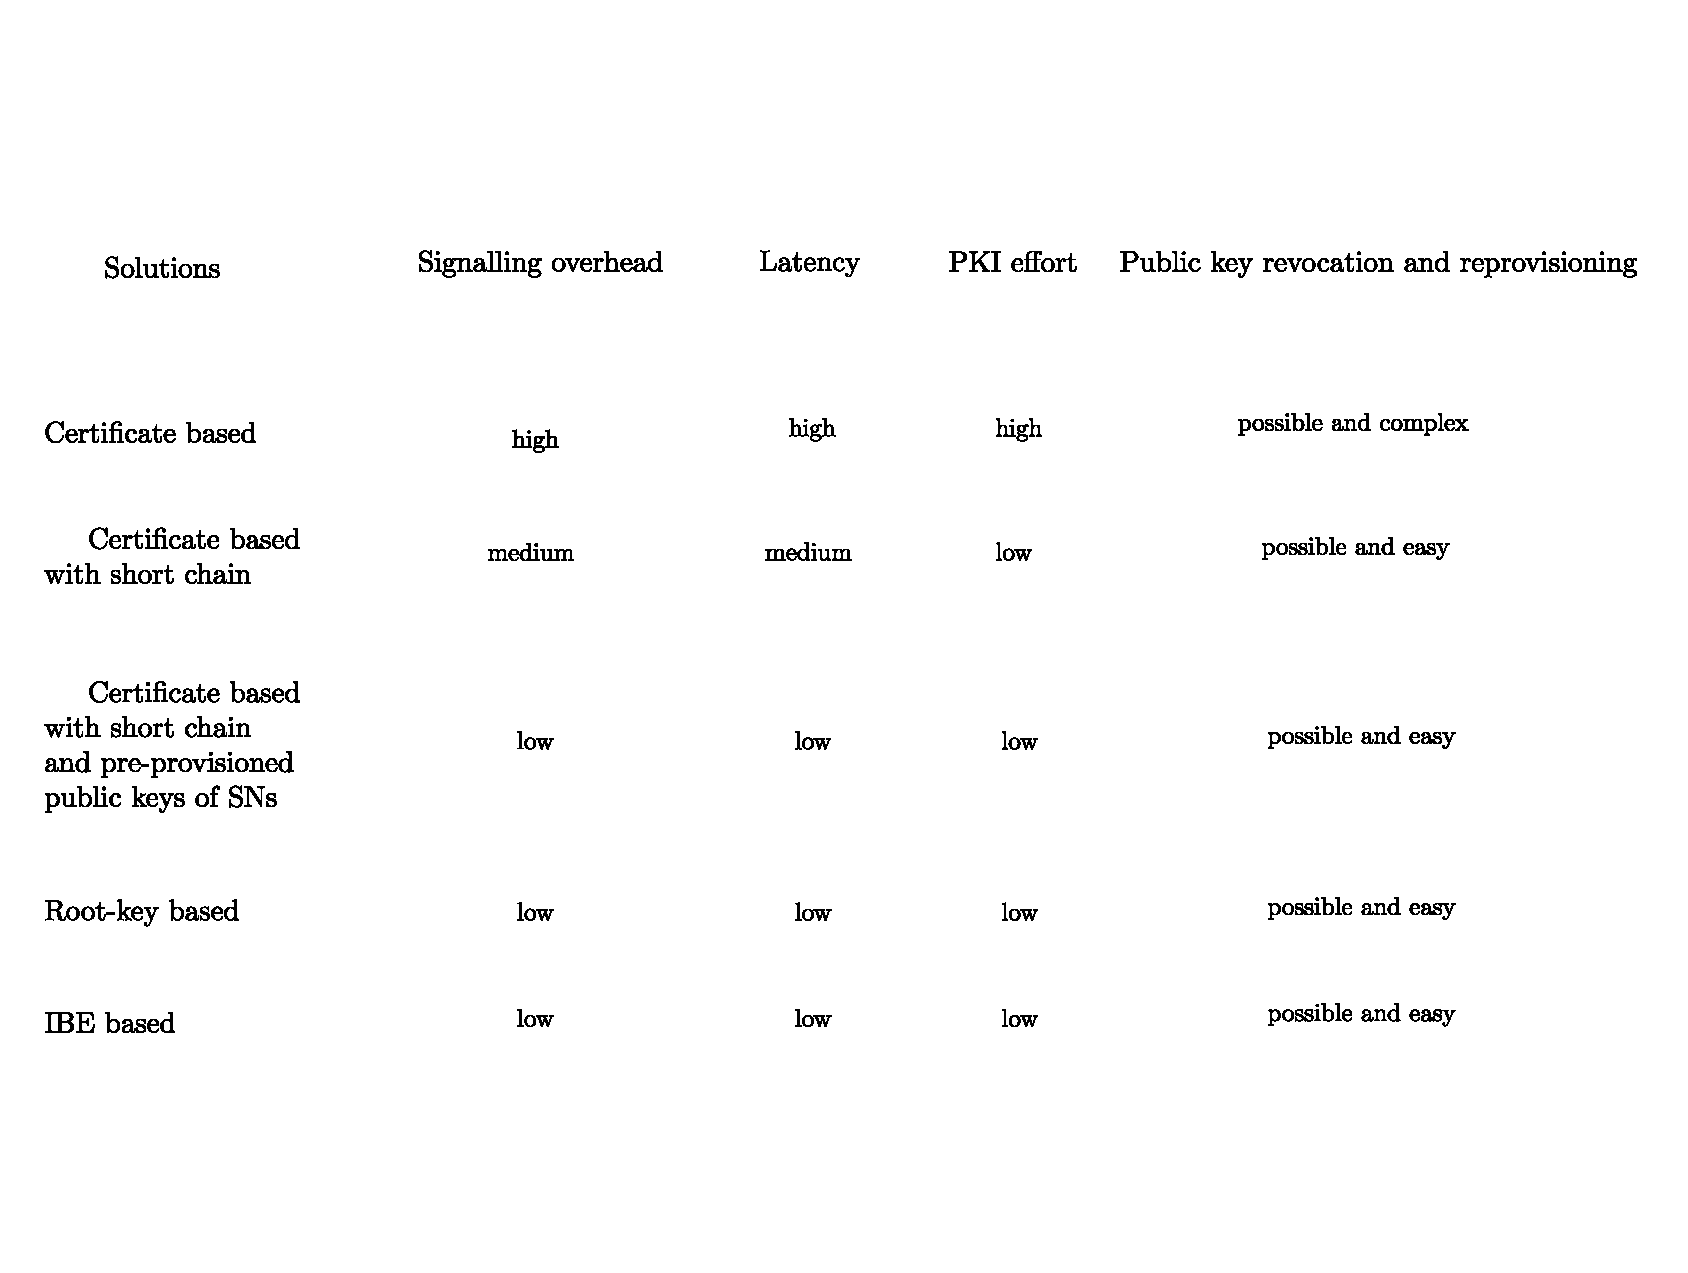
\includegraphics[width=.98\textwidth]{compare.eps}
% figure caption is below the figure
\caption{Comparison among the solutions}
\label{fig:solution_ibc}       % Give a unique label
\end{center}
\end{figure}
\paragraph{}
All the solutions are based on public-key encryption. As a result all of them requires expensive computation of public-key encryption. Another downside of public-key encryption is the size of the ciphertext is comparatively large. These two downsides will affect the latency and signalling overhead. Once a UE is identified and authenticated by the SN, the SN assigns a GUTI to the UE. In the consecutive identification and authentication, this GUTI can be used. However, when the GUTI is not synchronised in between the SN and the UE, or the UE tries to connect to a new SN, the GUTI does not work. In that situation, the solutions we have proposed can be used. Hence, solutions of public-key encryption based solution is not required to run each time there is a need of identification of a UE. By using a temporary identifier assigned to the UE by the HN, we can reduce the need of running the public-key encryption based solution. The temporary identifier assigned by the HN is called pseudonym. Solutions based on pseudonyms have been proposed in \cite{pseudonym_valtteri_philip,pseudonym_ericsson}. By using the public-key encryption based solution in conjunction with GUTI and pseudonym, the need for running the public-key encryption based solution becomes very infrequent. Besides, the need of low latency is mostly for making the tactile internet successful. As a result, it is the data plane where the low latency is critical, not the control plane. However, it is still a matter of further research to quantify the impact of public-key encryption on signalling overhead and latency. 



\section{Conclusion}
\label{sec:conclusion}
In this report we have discussed different solutions based on public-key encryption to protect the privacy of the long-term identifier known as IMSI. We have come up with a categorisation of public-key encryption and presented one solution using each of the subcategories. The comparative analysis among the techniques from different categories of public-key encryption shows that pre-provisioned public keys of the SNs, root-key and IBE based solutions are promising approaches to protect the IMSI privacy.
Interestingly, none of the solutions need a new entity to build the PKI. However, as all the solutions are based on public-key encryption, the expensive computation and longer ciphertext are the inherent downsides of all the solutions. These downsides affect the latency and signalling overhead. In conjunction with GUTI and pseudonym the impact on latency and signalling overhead can be reduced to large extent. However, quantification of the latency and signalling overhead remains open to further research.

\section{Acknowledgement}
\label{sec:acknowledgement}



\begin{thebibliography}{4}

\bibitem{NGMN_white_paper} NGMN 5G White Paper V1.0 [cited Jan, 2017]. Available at: https://www.ngmn.org/uploads/media/NGMN\_5G\_White\_Paper\_V1\_0.pdf

\bibitem{TR33899} 3GPP TR 33.899 V0.6.0 [cited Jan, 2017]. Available at: https://portal.3gpp.org/desktopmodules/Specifications/SpecificationDetails.aspx?\\specificationId=3045

\bibitem{TS23003} 3GPP TS 23.003 V14.2.0 [cited Jan, 2017]. Available at: https://portal.3gpp.org/desktopmodules/Specifications/SpecificationDetails.aspx?\\specificationId=729

\bibitem{TR21905} 3GPP TR 21.905 [cited Jan, 2017]. Available at: https://portal.3gpp.org/desktopmodules/Specifications/SpecificationDetails.aspx?\\specificationId=558


\bibitem{pseudonym_ericsson} Karl Norrman, Mats N\"aslund, Elena Dubrova: Protecting IMSI and User Privacy in 5G Networks. 2nd International Workshop on 5G Security

\bibitem{pseudonym_valtteri_philip} Philip Ginzboorg,  Valtteri Niemi: Privacy of the long-term identities in cellular networks. Proceedings of the 9th EAI International Conference on Mobile Multimedia Communications
Pages 167-175




\end{thebibliography}

\end{document}
